% Creating a simple Title Page in Beamer
\documentclass{beamer}

% Theme choice:
\usetheme{AnnArbor}

% Change numbers style
\usepackage{enumitem}

% customize the caption
\setbeamerfont{caption}{size=\large}
\setbeamercolor{caption}{fg=blue}
\setbeamercolor{caption name}{fg=red}

% Title page details:
\title{Introduction to Topology}
\author{yuzuki}
\institute{Eyes, Japan}
\date{\today}
\logo{
  
\includegraphics[width=3cm]{eyes-japan-logo.png}
}

\begin{document}

% Title page frame
\begin{frame}
  \titlepage
\end{frame}

% Outline frame
\begin{frame}{Outline}
  \tableofcontents
\end{frame}

% Current section
\AtBeginSection[ ]
{
  \begin{frame}{Outline}
    \tableofcontents[currentsection]
  \end{frame}
}

% Presentation structure
\section{Euler's theorem}

\begin{frame}{Euler's theorem}
  \begin{columns}
    % Column 1
    \begin{column}{0.5\textwidth}
      \begin{block}{}
        \begin{itemize}
        \item v: The number of vertices.
        \item e: The number of edges.
        \item f: The number of faces.
        \end{itemize}
      \end{block}
      \begin{block}{}
        $v - e + f = 2$
      \end{block}
      \begin{block}{}
        \begin{itemize}
        \item convex
        \item not convex
        \end{itemize}
      \end{block}
    \end{column}
    % Column 2
    \begin{column}{0.5\textwidth}
      \begin{figure}
        \centering
        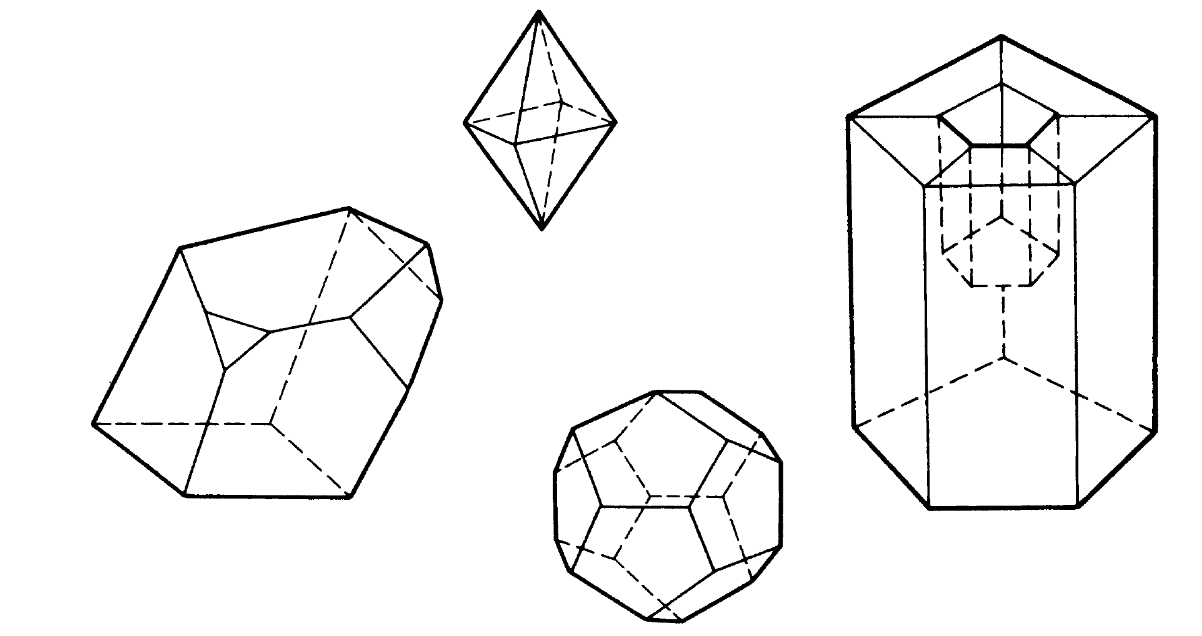
\includegraphics[width=0.7\textwidth]{figure_1_1.png}
        \caption{Polyhedra}
      \end{figure}
    \end{column}
  \end{columns}
\end{frame}

\begin{frame}{Euler's theorem}
  \begin{columns}
    % Column 1
    \begin{column}{0.5\textwidth}
      \begin{block}{}
        \begin{itemize}
        \item A polyhedron whose surface consists of two distinct pieces.
        \item Its surface is not connected.
        \item Each of the pieces of surface contributes 2 to $v - e + f$.
        \end{itemize}
      \end{block}
      \begin{block}{}
        $v - e + f = 4$
      \end{block}
    \end{column}
    % Column 2
    \begin{column}{0.5\textwidth}
      \begin{figure}
        \centering
        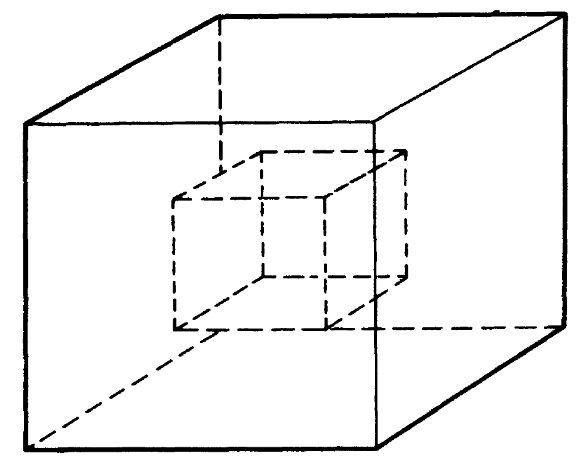
\includegraphics[width=0.7\textwidth]{figure_1_2.png}
        \caption{A cube with a small cube removed from its interior}
      \end{figure}
    \end{column}
  \end{columns}
\end{frame}

\begin{frame}{Euler's theorem}
  \begin{columns}
    % Column 1
    \begin{column}{0.5\textwidth}
      \begin{block}{}
        \begin{itemize}
        \item A polyhedron whose surface consists of all one piece.
        \item Can find a loop on the surface which does not separate it into two distinct parts.
        \item Imagine: Cutting round the loop with a pair of scissors, then the surface does not fall into two pieces.
        \end{itemize}
      \end{block}
      \begin{block}{}
        $v - e + f = 0$
      \end{block}
    \end{column}
    % Column 2
    \begin{column}{0.5\textwidth}
      \begin{figure}
        \centering
        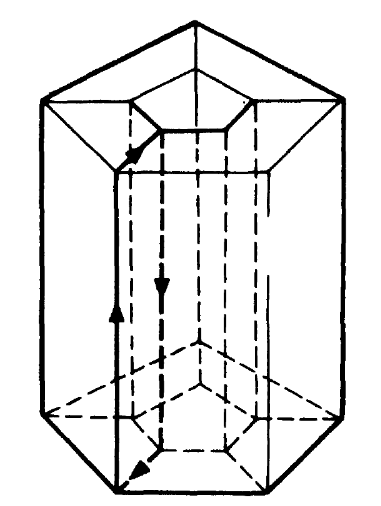
\includegraphics[width=0.7\textwidth]{figure_1_3.png}
        \caption{A prism with a hole straight through the centre}
      \end{figure}
    \end{column}
  \end{columns}
\end{frame}

\begin{frame}{Euler's theorem}
  \begin{columns}
    % Column 1
    \begin{column}{0.4\textwidth}
      \begin{block}{}
        \begin{itemize}
        \item The surfaces of solids (except, that is, when we mentioned convexity).
        \item Use the word polyhedron for such a surface, rather than for the solid which it bounds.
        \item A \textsl{polyhedron} is a finite collection of plane polygons which fit together nicely in the rigth sense:
        \end{itemize}
      \end{block}
    \end{column}
    % Column 2
    \begin{column}{0.6\textwidth}
      \begin{block}{}
        \begin{itemize}
        \item If two polygons meet they do so in a common edge, and each edge of a polygon lies in precisely one other polygon.
        \item In addition, we ask that if we consider the polygons which contain a particular vertex, then we can label them $Q_1$, $Q_2$,....,$Q_k$ in such a way that $Q_i$ has an edge in common with $Q_{i+1}$ for $1 \leq i < k$, and $Q_k$ has an edge in common with $Q_1$.
        \item In other words, the polygons fit together to form a piece of surface around the given vertex (The number \textsl{k} may vary from one vertex to another).
        \end{itemize}
      \end{block}
    \end{column}
  \end{columns}
\end{frame}

\begin{frame}{Euler's theorem}
  % Theorem environment
  \begin{theorem}[(1.1) Euler's theorem.]
    Let P be a polyhedron which satisfies:
    \begin{enumerate}[label={(\alph*)}]
    \item Any two vertices of P can be connected by a chain of edges.
    \item Any loop on P which is made up of straight line segments (not necessary edges) separates P into two pieces.
    \end{enumerate}
    Then v - e + f = 2 for P.
  \end{theorem}
\end{frame}

\begin{frame}{Euler's theorem}
  \begin{columns}
    % Column 1
    \begin{column}{0.5\textwidth}
      \begin{definition}[Graph]
        A connected set of vertices and edges of \textsl{P}.
        \begin{itemize}
        \item Connected simply means that any two vertices can be joined by a chain of edges in the graph.
        \item We use the word graph for any finite connected set of line segments in 3-space which fit together nicely as the right figure.
        \item If two segments intersect they are required to do so in a common vertex.
        \end{itemize}
      \end{definition}
    \end{column}
    % Column 2
    \begin{column}{0.5\textwidth}
      \begin{figure}
        \centering
        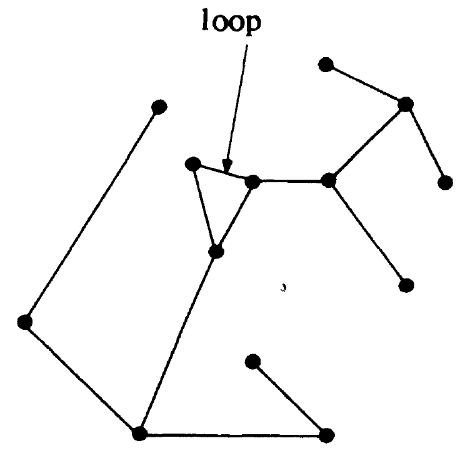
\includegraphics[width=0.7\textwidth]{figure_1_4_b.png}
        \caption{Graph}
      \end{figure}
    \end{column}
  \end{columns}
\end{frame}

\begin{frame}{Euler's theorem}
  \begin{columns}
    % Column 1
    \begin{column}{0.5\textwidth}
      \begin{definition}[Tree]
        A graph which does not contain any loops.
        \begin{itemize}
        \item For a tree, the number of vertices minus the number of edges is equal to 1.
        \item If the tree is denoted by \textsl{T}, we shall write this as $v(T) - e(T) = 1$.
        \end{itemize}
      \end{definition}
    \end{column}
    % Column 2
    \begin{column}{0.5\textwidth}
      \begin{figure}
        \centering
        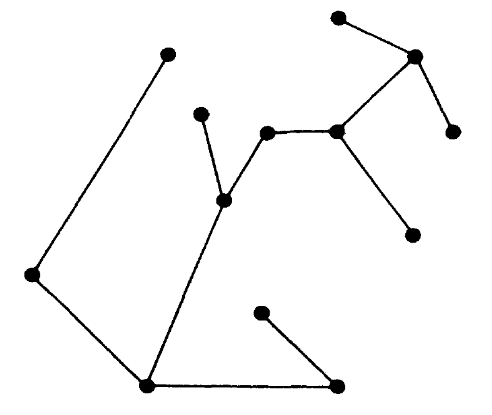
\includegraphics[width=0.7\textwidth]{figure_1_4_a.png}
        \caption{Tree}
      \end{figure}
    \end{column}
  \end{columns}
\end{frame}

\begin{frame}{Euler's theorem}
  \begin{columns}
    % Column 1
    \begin{column}{0.5\textwidth}
      \begin{proof}
        \begin{itemize}
        \item The set of all vertices and edges of \textsl{P} is a graph.
        \item In any graph find a subgraph which is a tree and which contains all the vertices of the original.
        \item Choose a tree \textsl{T} which consists of some of the edges and all of the vertices of \textsl{P}.
        \end{itemize}
      \end{proof}
    \end{column}
    % Column 2
    \begin{column}{0.5\textwidth}
      \begin{figure}
        \centering
        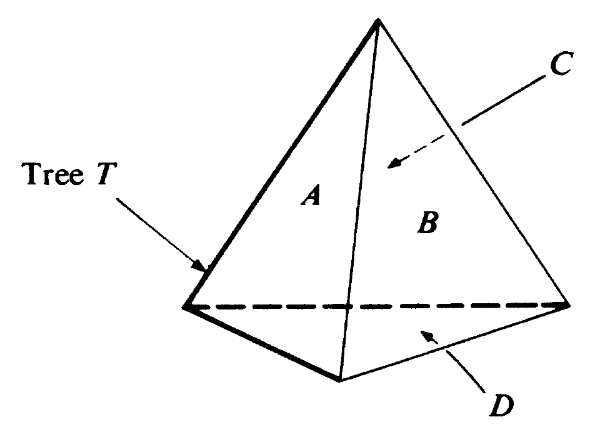
\includegraphics[width=0.7\textwidth]{figure_1_5_a.png}
        \caption{Subgraph-Tree}
      \end{figure}
    \end{column}
  \end{columns}
\end{frame}

\begin{frame}{Euler's theorem}
  \begin{columns}
    % Column 1
    \begin{column}{0.6\textwidth}
      \begin{proof}
        Form a sort of dual to \textsl{T}. This dual is a grap $\Gamma$ defined as follows:
        \begin{itemize}
        \item For each face \textsl{A} of \textsl{P} we give $\Gamma$ a vertex $\hat A$.
        \item Two vertices $\hat A$ and $\hat B$ of $\Gamma$ are joined by an edge if and only if the corresponding faces \textsl{A} and \textsl{B} of \textsl{P} are adjacent with intersection an edge that is not in \textsl{T}.
        \item The vertex $\hat A$ corresponding to an interior point of \textsl{A}.
        \item We allow the edges of $\Gamma$ to be bent.
        \end{itemize}
      \end{proof}
    \end{column}
    % Column 2
    \begin{column}{0.4\textwidth}
      \begin{figure}
        \centering
        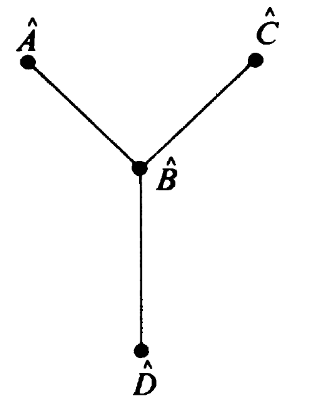
\includegraphics[width=0.7\textwidth]{figure_1_5_b.png}
        \caption{Associated tree $\Gamma$}
      \end{figure}
    \end{column}
  \end{columns}
\end{frame}

\begin{frame}{Euler's theorem}
  \begin{columns}
    % Column 1
    \begin{column}{0.6\textwidth}
      \begin{proof}
        Dual $\Gamma$ is connected and is therefore a graph.
        \begin{itemize}
        \item Intuitively, if two vertices of $\Gamma$ cannot be connected by a chain of edges of $\Gamma$, then they must be separated from one another by a loop of \textsl{T}.
        \item Since \textsl{T} does not contain any loops we deduce that $\Gamma$ must be connected.
        \end{itemize}
      \end{proof}
    \end{column}
    % Column 2
    \begin{column}{0.4\textwidth}
      \begin{figure}
        \centering
        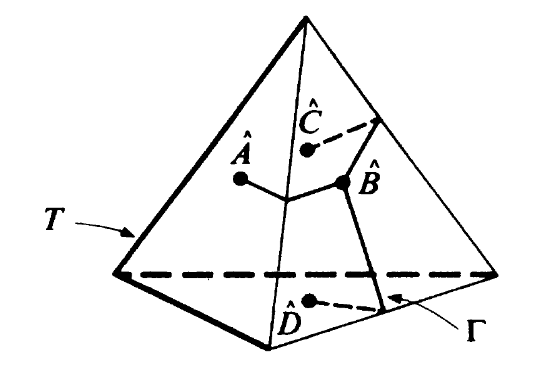
\includegraphics[width=0.7\textwidth]{figure_1_5_c.png}
        \caption{Associated tree $\Gamma$}
      \end{figure}
    \end{column}
  \end{columns}
\end{frame}

\begin{frame}{Euler's theorem}
  \begin{columns}
    % Column 1
    \begin{column}{0.6\textwidth}
      \begin{proof}
        In fact $\Gamma$ is a tree.
        \begin{itemize}
        \item For if there were a loop in $\Gamma$ it would separate \textsl{P} into two distinct pieces by hypothesis (b), and each of these pieces must contain at least one vertex of $\Gamma$.
        \item Any attempt to connect two vertices of \textsl{T} which lie in different pieces by a chain of edges results in a chain which  meets this separating loop, and therefore in a chain which cannot lie entirely in \textsl{T}.
        \item This contradicts the fact that \textsl{T} is connected. Therefore $\Gamma$ is a tree.
        \end{itemize}
      \end{proof}
    \end{column}
    % Column 2
    \begin{column}{0.4\textwidth}
      \begin{figure}
        \centering
        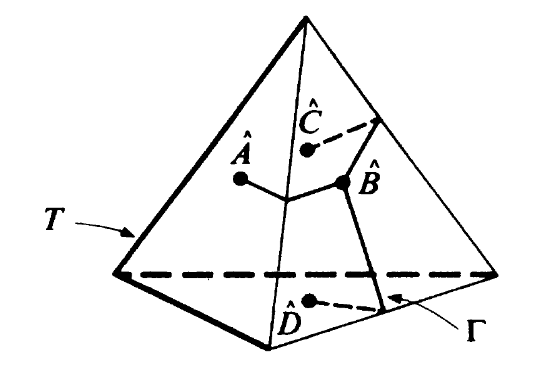
\includegraphics[width=0.7\textwidth]{figure_1_5_c.png}
        \caption{Associated tree $\Gamma$}
      \end{figure}
    \end{column}
  \end{columns}
\end{frame}

\begin{frame}{Euler's theorem}
  \begin{columns}
    % Column 1
    \begin{column}{0.6\textwidth}
      \begin{proof}
        \begin{itemize}
        \item Since $v(T) - e(T) = 1$ and $v(\Gamma) - e(\Gamma) = 1$.
        \item Therefore $v(T) - [e(T) + e(\Gamma)] + v(\Gamma) = 2$.
        \item By construction $v(T) = v$, $e(T) + e(\Gamma) = e$, $v(\Gamma) = f$.
        \end{itemize}
      \end{proof}
    \end{column}
    % Column 2
    \begin{column}{0.4\textwidth}
      \begin{figure}
        \centering
        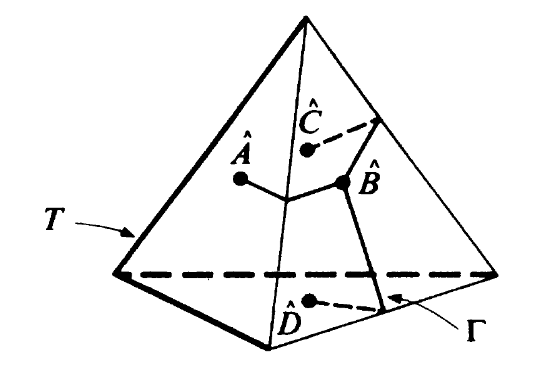
\includegraphics[width=0.7\textwidth]{figure_1_5_c.png}
        \caption{Associated tree $\Gamma$}
      \end{figure}
    \end{column}
  \end{columns}
\end{frame}

\section{Topological equivalence}

\begin{frame}{Topological equivalence}
  \begin{columns}
    \begin{column}{0.6\textwidth}
      \begin{block}{}
        The proof contains more information:
        \begin{itemize}
        \item \textsl{P} is made up of two discs which are identified along their boundaries.
        \item Thicken each of \textsl{T} and $\Gamma$ a little on \textsl{P} to obtain two disjoint discs.
        \item Thickening a tree always gives a disc, thickening a graph with loops will give a space with holes in it.
        \item Enlarge these discs little by little until their boundaries coincide.
        \item The polyhedron \textsl{P} is now made up of two discs which have a common boundary.
        \end{itemize}
      \end{block}
    \end{column}
    % Column 2
    \begin{column}{0.4\textwidth}
      \begin{figure}
        \centering
        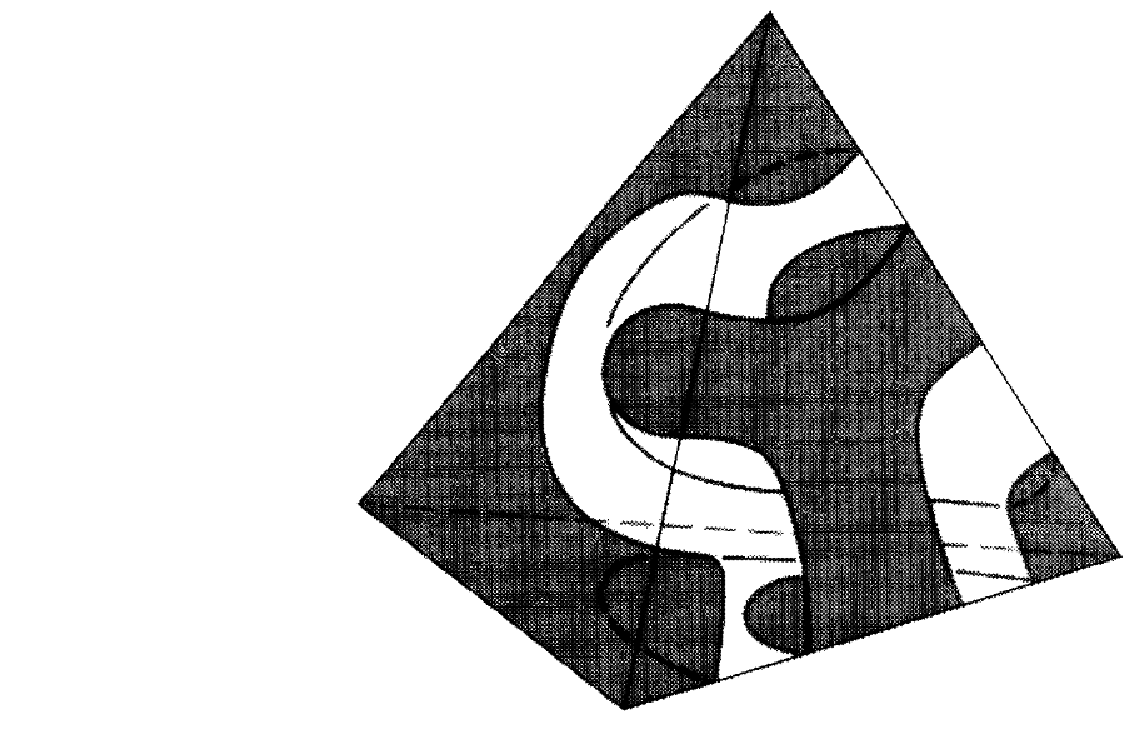
\includegraphics[width=0.7\textwidth]{figure_1_6.png}
        \caption{\textsl{T} and $\Gamma$ thickened on \textsl{P}}
      \end{figure}
    \end{column}
  \end{columns}
\end{frame}

\begin{frame}{Topological equivalence}
  \begin{columns}
    \begin{column}{0.6\textwidth}
      \begin{block}{}
        \begin{itemize}
        \item Granted these discs may have a rather odd shape, but they can be deformed into ordinary, round flat discs.
        \end{itemize}
      \end{block}
    \end{column}
    % Column 2
    \begin{column}{0.4\textwidth}
      \begin{figure}
        \centering
        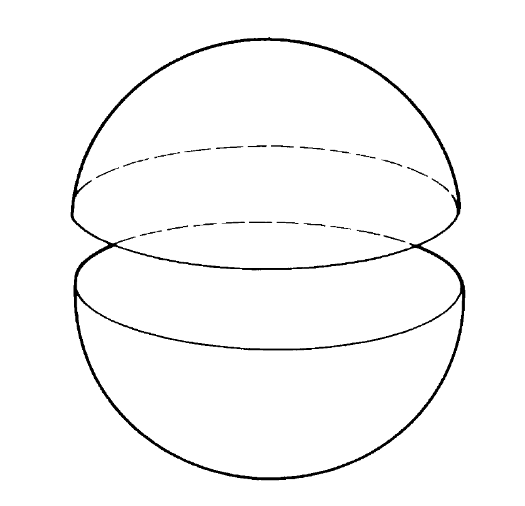
\includegraphics[width=0.7\textwidth]{figure_1_7.png}
        \caption{}
      \end{figure}
    \end{column}
  \end{columns}
\end{frame}

\begin{frame}{Topological equivalence}
  \begin{columns}
    \begin{column}{0.6\textwidth}
      \begin{block}{}
        \begin{itemize}
        \item The sphere consists of two discs, the north and south hemispheres, sewn along their common boundary the equator.
        \item In other words, the hypotheses of Euler's theorem tell us that \textsl{P} looks in some sense like a rather deformed sphere.
        \end{itemize}
      \end{block}
    \end{column}
    % Column 2
    \begin{column}{0.4\textwidth}
      \begin{figure}
        \centering
        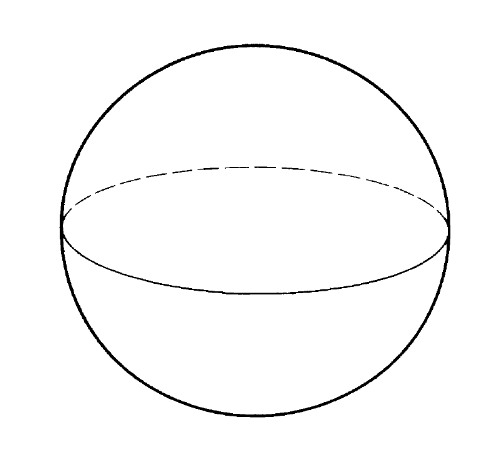
\includegraphics[width=0.7\textwidth]{figure_1_7_b.png}
        \caption{identify boundaries}
      \end{figure}
    \end{column}
  \end{columns}
\end{frame}

\begin{frame}{Topological equivalence}
  \begin{columns}
    \begin{column}{0.6\textwidth}
      \begin{block}{}
        For a specific polyhedron it may be very easy to set up a decent correspondence bwtween its points and those of the sphere.
        \begin{itemize}
        \item For example, in the case of the regular tetrahedron \textsl{T} we can use radial projection from the centre of gravity $\hat T$ of \textsl{T} to project \textsl{T} onto a sphere with centre $\hat T$.
        \end{itemize}
      \end{block}
    \end{column}
    % Column 2
    \begin{column}{0.4\textwidth}
      \begin{figure}
        \centering
        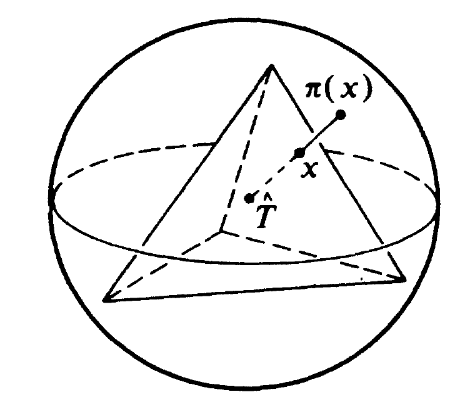
\includegraphics[width=0.7\textwidth]{figure_1_8_a.png}
        \caption{Radial projection $\pi$}
      \end{figure}
    \end{column}
  \end{columns}
\end{frame}

\begin{frame}{Topological equivalence}
  \begin{columns}
    \begin{column}{0.6\textwidth}
      \begin{block}{}
        \begin{itemize}
        \item The faces of \textsl{T} project to curvilinear triangles on the sphere as shown on the right fig.
        \end{itemize}
      \end{block}
    \end{column}
    % Column 2
    \begin{column}{0.4\textwidth}
      \begin{figure}
        \centering
        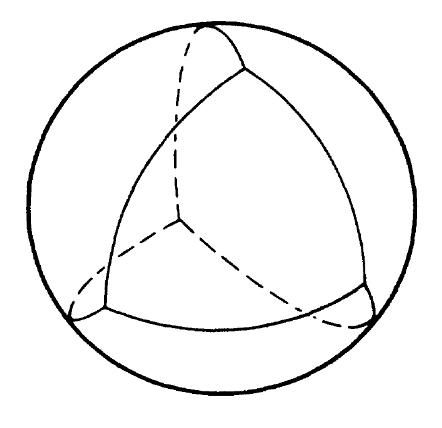
\includegraphics[width=0.7\textwidth]{figure_1_8_b.png}
        \caption{Radial projection $\pi$}
      \end{figure}
    \end{column}
  \end{columns}
\end{frame}

\begin{frame}{Topological equivalence}
  \begin{columns}
    % Column 1
    \begin{column}{0.6\textwidth}
      \begin{block}{}
        \begin{itemize}
        \item The polyhedron that is not convex does not lend itself to the above argument.
        \item However, if we think of it as being made of rubber then we can easily imagine how to deform it into an ordinary round sphere.
        \item During the deformation we stretch and bend the polyhedron at will, \textsl{but we never identify distinct points and we never tear it}.
        \end{itemize}
      \end{block}
    \end{column}
    % Column 2
    \begin{column}{0.4\textwidth}
      \begin{figure}
        \centering
        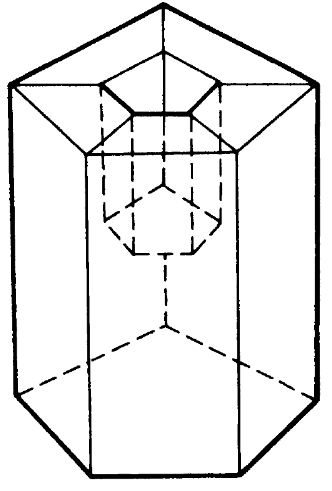
\includegraphics[width=0.7\textwidth]{figure_1_8_c.png}
        \caption{Polyhedron that is not convex}
      \end{figure}
    \end{column}
  \end{columns}
\end{frame}

\begin{frame}{Topological equivalence}
  \begin{columns}
    % Column 1
    \begin{column}{1.0\textwidth}
      \begin{block}{}
        \begin{itemize}
        \item The resulting correspondence between the points of the given polyhedron and the points of the sphere is an example of \textsl{topological equivalence} or \textsl{homeomorphism}.
        \item In formal terms it is a one-one and onto continuous function with continuous inverse.
        \end{itemize}
      \end{block}
    \end{column}
  \end{columns}
\end{frame}

\begin{frame}{Topological equivalence}
  \begin{block}{}
    To help make things a little more concrete: Here are four spaces which are homeomorphic.
  \end{block}
  \begin{columns}
    \begin{column}{0.4\textwidth}
      \begin{figure}
        \centering
        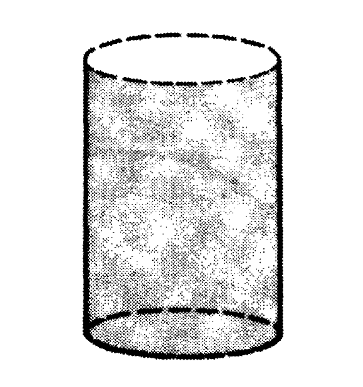
\includegraphics[width=0.7\textwidth]{figure_1_9_a.png}
        \caption{(a) Surface of cylinder finite height, excluding the two circles at the ends}
      \end{figure}
    \end{column}
    % Column 2
    \begin{column}{0.6\textwidth}
      \begin{figure}
        \centering
        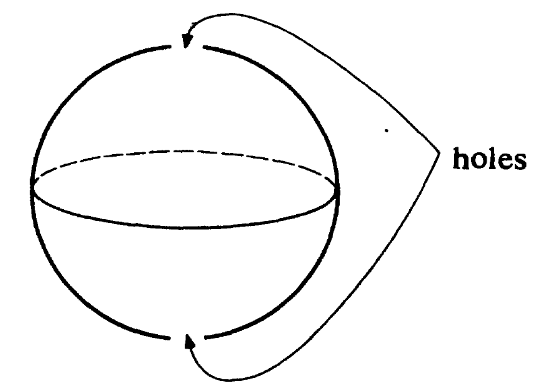
\includegraphics[width=0.7\textwidth]{figure_1_9_d.png}
        \caption{(b) Sphere with the points at the north and south poles removed}
      \end{figure}
    \end{column}
  \end{columns}
\end{frame}

\begin{frame}{Topological equivalence}
  \begin{block}{}
    To help make things a little more concrete: Here are four spaces which are homeomorphic.
  \end{block}
  \begin{columns}
    \begin{column}{0.5\textwidth}
      \begin{figure}
        \centering
        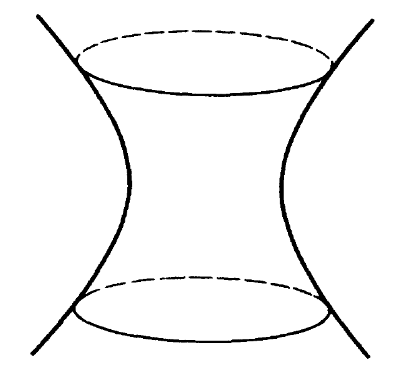
\includegraphics[width=0.7\textwidth]{figure_1_9_b.png}
        \caption{(c) One-sheeted hyperboloid given by the equation $x^2 + y^2 - z^2 = 1$}
      \end{figure}
    \end{column}
    % Column 2
    \begin{column}{0.5\textwidth}
      \begin{figure}
        \centering
        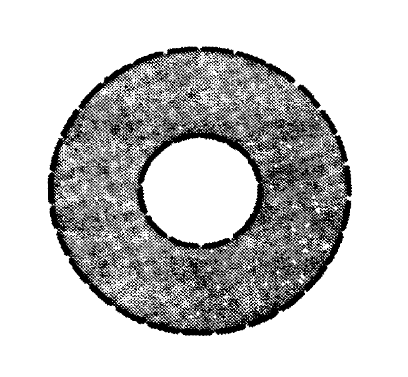
\includegraphics[width=0.7\textwidth]{figure_1_9_c.png}
        \caption{(d) Open annulus in the complex plane specified by $1 < |z| < 3$}
      \end{figure}
    \end{column}
  \end{columns}
\end{frame}

\section{Surfaces}

\begin{frame}{Surfaces}
  \begin{block}{}
    Being geometers at heart, we are more interested in bounded configurations which occure natually in euclidean space. For example, the unit circle, the unit disc in the plane, surfaces such as:
  \end{block}
  \begin{columns}
    \begin{column}{0.5\textwidth}
      \begin{figure}
        \centering
        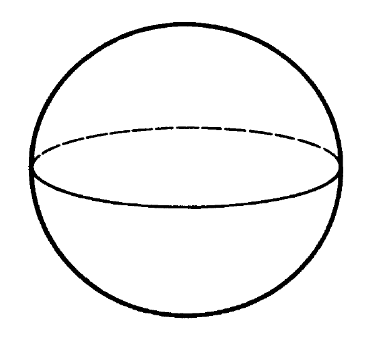
\includegraphics[width=0.7\textwidth]{figure_1_10_a.png}
        \caption{(a) Sphere}
      \end{figure}
    \end{column}
    % Column 2
    \begin{column}{0.5\textwidth}
      \begin{figure}
        \centering
        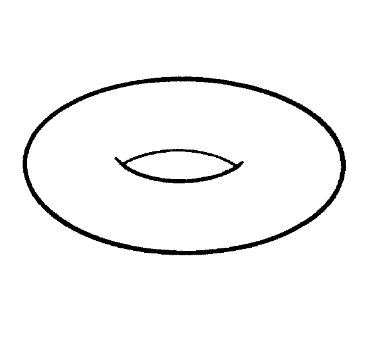
\includegraphics[width=0.7\textwidth]{figure_1_10_b.png}
        \caption{(b) Torus}
      \end{figure}
    \end{column}
  \end{columns}
\end{frame}

\begin{frame}{Surfaces}
  \begin{block}{}
    All of which live in three-dimensional space.
  \end{block}
  \begin{columns}
    \begin{column}{0.5\textwidth}
      \begin{figure}
        \centering
        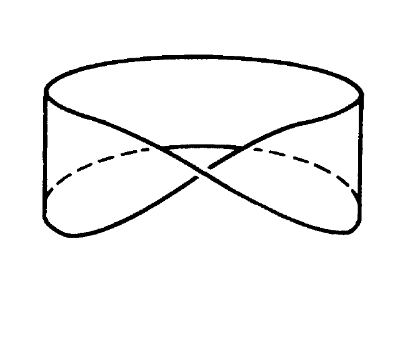
\includegraphics[width=0.7\textwidth]{figure_1_10_c.png}
        \caption{(c) Mobius strip}
      \end{figure}
    \end{column}
    % Column 2
    \begin{column}{0.5\textwidth}
      \begin{figure}
        \centering
        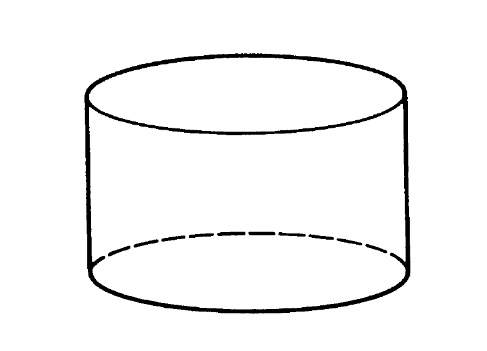
\includegraphics[width=0.7\textwidth]{figure_1_10_d.png}
        \caption{(d) Cylinder}
      \end{figure}
    \end{column}
  \end{columns}
\end{frame}

\begin{frame}{Surfaces}
  \begin{block}{}
    Klein bottle is difficult to imagine because in any attempt to represent it in three dimensions the Klein bottle must cross itself. In our drawing the surface cuts itself in a small circle.
  \end{block}
  \begin{columns}
    \begin{column}{0.5\textwidth}
      \begin{figure}
        \centering
        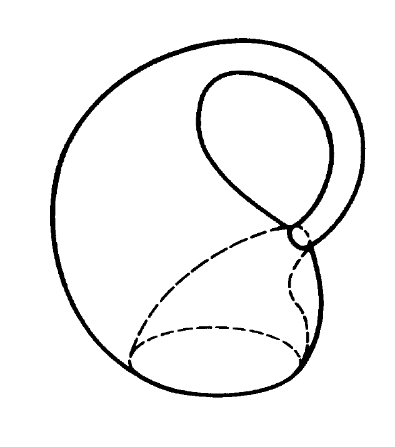
\includegraphics[width=0.7\textwidth]{figure_1_10_e.png}
        \caption{(e) Klein bottle}
      \end{figure}
    \end{column}
    % Column 2
    \begin{column}{0.5\textwidth}
      \begin{figure}
        \centering
        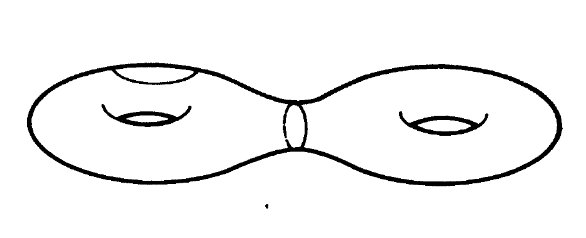
\includegraphics[width=0.7\textwidth]{figure_1_10_f.png}
        \caption{(f) Punctured double torus}
      \end{figure}
    \end{column}
  \end{columns}
\end{frame}

\begin{frame}{Surfaces}
  \begin{block}{}
    To build a Klein bottle, the first half of the construction, that is as far as cylinder, is the same.
  \end{block}
  \begin{figure}
    \centering
    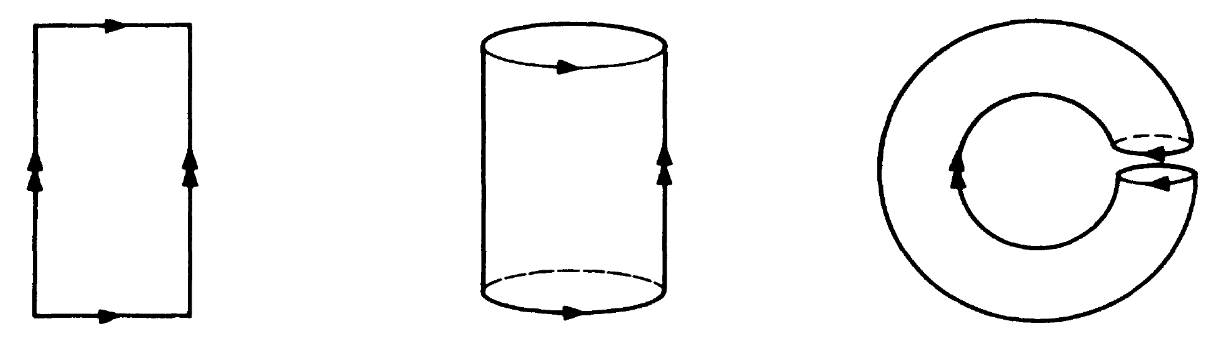
\includegraphics[width=0.7\textwidth]{figure_1_11.png}
    \caption{}
  \end{figure}
\end{frame}

\begin{frame}{Surfaces}
  \begin{block}{}
    But then the ends of the cylinder are identified in the opposite direction. In order to do this, the cylinder has to be bent around and one end pushed through the side as in the Fig.
  \end{block}
  \begin{figure}
    \centering
    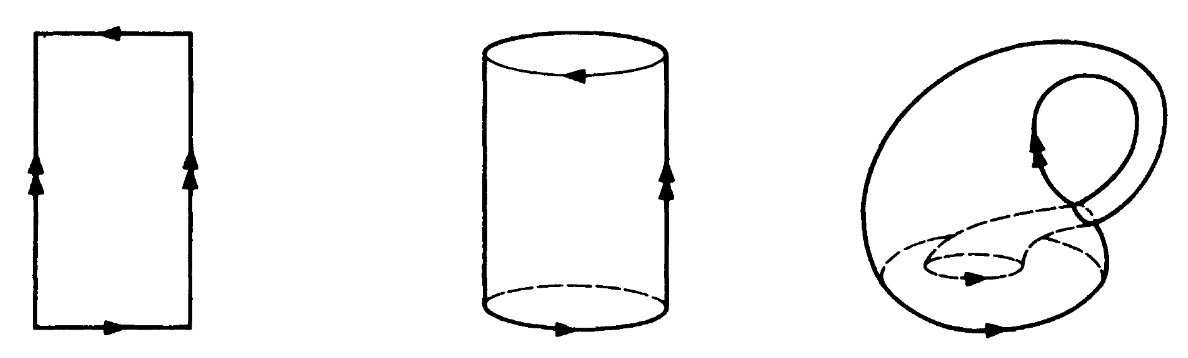
\includegraphics[width=0.7\textwidth]{figure_1_12.png}
    \caption{}
  \end{figure}
\end{frame}

\begin{frame}{Surfaces}
  \begin{block}{}
    The Klein bottle (\textsl{K}) can be represented in four-dimensional space without any self intersections.
    \begin{itemize}
    \item Imagine an extra dimension perpendicular to the paper, remembering all the time that the paper represents ordinary three-dimensional space.
    \item Near the intersection circle of \textsl{K} we have two pipes, one of which cuts through the other.
    \item Lift one pipe a little clear of the other into the fourth dimension.
    \end{itemize}
  \end{block}
  \begin{figure}
    \centering
    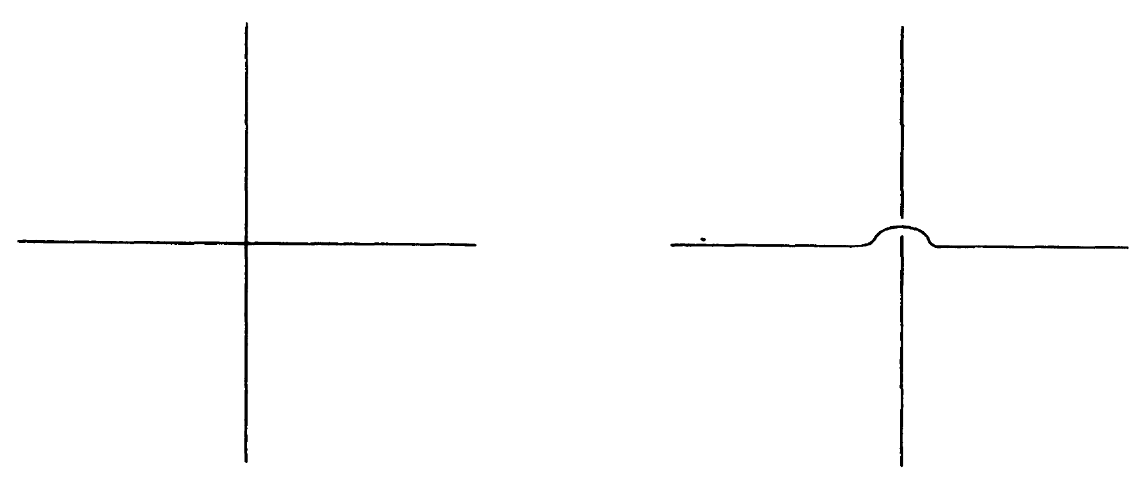
\includegraphics[width=0.7\textwidth]{figure_1_13.png}
    \caption{}
  \end{figure}
\end{frame}

\begin{frame}{Surfaces}
  \begin{block}{}
    Our way of introducing surfaces by representing them in euclidean space is not such a good idea as it might appear at first sight.
  \end{block}
\end{frame}

\begin{frame}{Surfaces}
  \begin{block}{}
    Three copies of the Mobius strip \textsl{M}. (a) and (b) are homeomorphic is no surprise, one only has to take a rubber version of (a) and stretch it into the (b)
  \end{block}
  \begin{columns}
    \begin{column}{0.5\textwidth}
      \begin{figure}
        \centering
        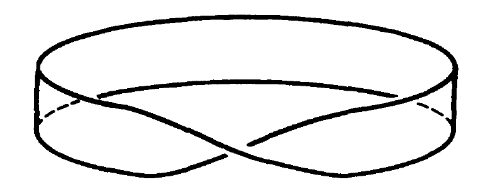
\includegraphics[width=0.7\textwidth]{figure_1_14_a.png}
        \caption{(a)}
      \end{figure}
    \end{column}
    % Column 2
    \begin{column}{0.5\textwidth}
      \begin{figure}
        \centering
        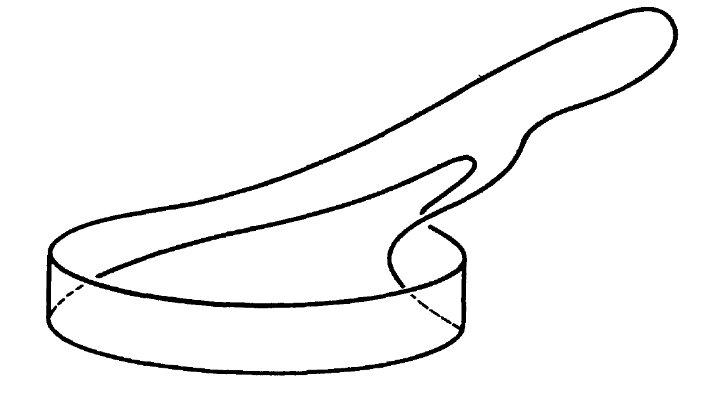
\includegraphics[width=0.7\textwidth]{figure_1_14_b.png}
        \caption{(b)}
      \end{figure}
    \end{column}
  \end{columns}
\end{frame}

\begin{frame}{Surfaces}
  \begin{block}{}
    \begin{itemize}
    \item But how about (a) and (c)?
    \item These spaces are homeomorphic, yet no amount of stretching, bending, and twisting will deform one into the other.
    \item To show two spaces are homeomorphic one must find a continous bijection between them, whose inverse is also continuous.
    \end{itemize}
  \end{block}
  \begin{columns}
    \begin{column}{0.5\textwidth}
      \begin{figure}
        \centering
        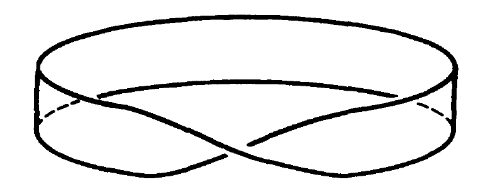
\includegraphics[width=0.7\textwidth]{figure_1_14_a.png}
        \caption{(a)}
      \end{figure}
    \end{column}
    % Column 2
    \begin{column}{0.5\textwidth}
      \begin{figure}
        \centering
        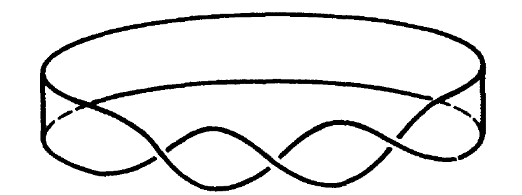
\includegraphics[width=0.7\textwidth]{figure_1_14_c.png}
        \caption{(c)}
      \end{figure}
    \end{column}
  \end{columns}
\end{frame}

\begin{frame}{Surfaces}
  \begin{block}{}
    Let's consider how to construct \textsl{M}.
    \begin{itemize}
    \item Buliding a model is easy: begin with a rectangle of paper and identify a pair of opposite edges with a half twist. This gives the usual representation of \textsl{M} as (a).
    \item To obtain (c) we must add a full twist to the above process.
    \end{itemize}
  \end{block}
  \begin{figure}
    \centering
    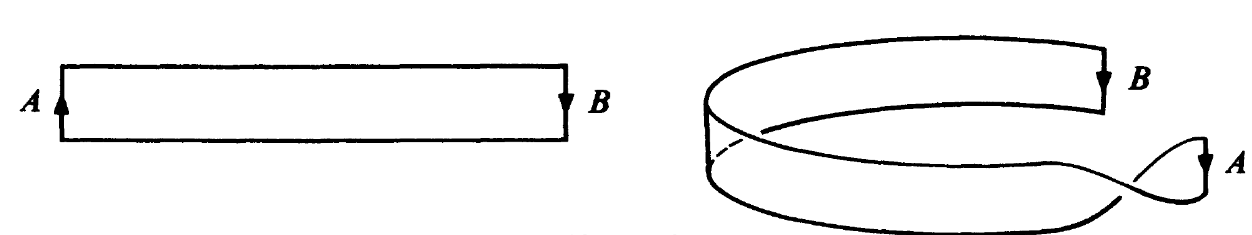
\includegraphics[width=0.7\textwidth]{figure_1_15.png}
    \caption{}
  \end{figure}
\end{frame}

\begin{frame}{Surfaces}
  \begin{block}{}
    \begin{itemize}
    \item But in terms of the identification of the edges A and B this changes nothing, the same points of A and B are made to coincide. Therefore the spaces (a) and (c) are homeomorphic.
    \item They are merely different representations of the \textsl{same} space in euclidean space.
    \item In other words, there is no homeomorphism from euclidean space to itself that throws (a) to (c).
    \end{itemize}
  \end{block}
  \begin{columns}
    \begin{column}{0.5\textwidth}
      \begin{figure}
        \centering
        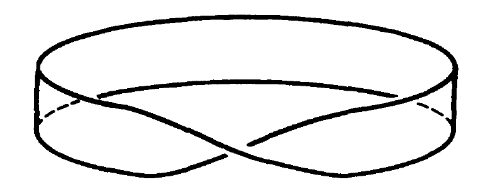
\includegraphics[width=0.7\textwidth]{figure_1_14_a.png}
        \caption{(a)}
      \end{figure}
    \end{column}
    % Column 2
    \begin{column}{0.5\textwidth}
      \begin{figure}
        \centering
        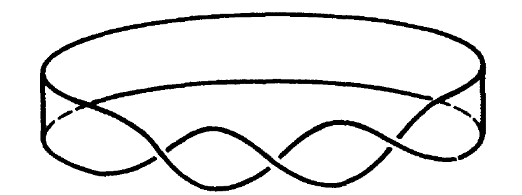
\includegraphics[width=0.7\textwidth]{figure_1_14_c.png}
        \caption{(c)}
      \end{figure}
    \end{column}
  \end{columns}
\end{frame}

\begin{frame}{Surfaces}
  \begin{block}{}
    \begin{itemize}
    \item This suggests very strongly that we need some way of considering our spaces abstractly rather than relying on particular representatives of them in euclidean space.
    \end{itemize}
  \end{block}
\end{frame}

\section{Abstract spaces}

\begin{frame}{Abstract spaces}
  \begin{block}{}
    Rephrase the classical definition of continuity as: \textsl{f} is continuous if given any x $\in$ $\mathbb{E}^m$ and any neighbourhood \textsl{N} of $f(x)$ in $\mathbb{E}^n$, then $f^{-1}(N)$ is a neighbourhood of x in $\mathbb{E}^n$.
  \end{block}
\end{frame}

\begin{frame}{Abstract spaces}
  \begin{block}{}
    Inspection of the properties of neighbourhoods of points in a euclidean space leads to the following axioms of a topological space.
  \end{block}
\end{frame}

\begin{frame}{Abstract spaces}
  % Theorem environment
  \begin{block}{}(1.2) We ask for a set \textsl{X} and for each point \textsl{x} of \textsl{X} a nonempty collection of subsets of \textsl{X}, called neighbourhoods. These neighbourhoods are required to satisfy four axioms:
    \begin{itemize}
    \item (a) \textsl{x} lies in each of its neighbourhoods.
    \item (b) The intersection of two neighbourhoods of \textsl{x} is itself a neighbourhood of \textsl{x}.
    \item (c) If \textsl{N} is a neighbourhood of \textsl{x} and if \textsl{U} is a subset of \textsl{X} which contains \textsl{N}, then \textsl{U} is a neighbourhood of \textsl{x}.
    \item (d) If \textsl{N} is a neighbourhood of x and if $\overset{\circ}{N}$ denotes the set {{$z \in N|N$ is a neighbourhood of $z$}}.
    \end{itemize}
  \end{block}
\end{frame}

\begin{frame}{Abstract spaces}
  \begin{definition}[Surface]
    (1.3) A surface is a topological space in which each point has a neighbourhood homeomorphic to the plane, and for which any two distinct points possess disjoint neighbourhoods.
    \begin{itemize}
    \item The definition fits exactly our intuitive idea of what a surface should be.
    \item If we stand in it at some point (imagining a giant version of the surface in question) and look at the points very close to our feet we should be able to imagine that we are standing on a plane.
    \item The surface of the earth is a good example. Unless you belong to the Flat Earth Society you believe it to be (topologically) a sphere, yet locailly it looks distinctly planar.
    \end{itemize}
  \end{definition}
\end{frame}

\section{A classification theorem}

\begin{frame}{A classification theorem}
  % Theorem environment
  \begin{theorem}[(1.4) Classification theorem.]
    Any closed surface is homeomorphic either to:
    \begin{enumerate}[label={(\alph*)}]
    \item The sphere.
    \item The sphere with a finite number (\textsl{n}) of handles added (an orientable surface of genus n).
    \item The sphere with a finite number of discs removed and replaced by Mobius strips(nonorientable).
    \end{enumerate}
    No two of these surfaces are homeomorphic.
  \end{theorem}
\end{frame}

\begin{frame}{A classification theorem}
  \begin{columns}
    % Column 1
    \begin{column}{0.6\textwidth}
      \begin{block}{}
        An orientable surface of genus n.
        \begin{itemize}
        \item If we draw a smooth closed curve on it,
        \item choose tangent and normal vectors at point (i.e., choose a coordinating system near the point -- often called a local orientation),
        \item and then push these vectors once round the curve
        \item we come back to the same system of vectors.
        \end{itemize}
      \end{block}
    \end{column}
    % Column 2
    \begin{column}{0.4\textwidth}
      \begin{figure}
        \centering
        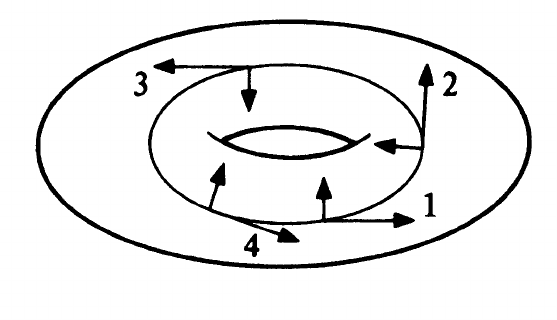
\includegraphics[width=0.7\textwidth]{figure_1_19_a.png}
        \caption{Polyhedron that is not convex}
      \end{figure}
    \end{column}
  \end{columns}
\end{frame}

\begin{frame}{A classification theorem}
  \begin{columns}
    % Column 1
    \begin{column}{0.6\textwidth}
      \begin{block}{}
        Nonorientable
        \begin{itemize}
        \item Any surface which contains a Mobius strip cannot satisfy this property.
        \item When we push tangent and normal vectors once round the central circle of the Mobius strip, the normal vector is reversed.
        \end{itemize}
      \end{block}
    \end{column}
    % Column 2
    \begin{column}{0.4\textwidth}
      \begin{figure}
        \centering
        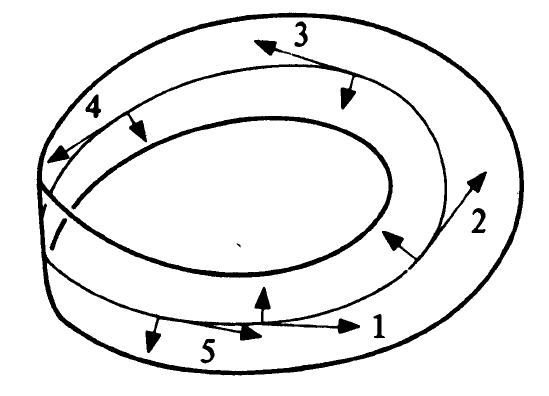
\includegraphics[width=0.7\textwidth]{figure_1_19_b.png}
        \caption{Polyhedron that is not convex}
      \end{figure}
    \end{column}
  \end{columns}
\end{frame}

\end{document}